%
% File acl2020.tex
%
%% Based on the style files for ACL 2020, which were
%% Based on the style files for ACL 2018, NAACL 2018/19, which were
%% Based on the style files for ACL-2015, with some improvements
%%  taken from the NAACL-2016 style
%% Based on the style files for ACL-2014, which were, in turn,
%% based on ACL-2013, ACL-2012, ACL-2011, ACL-2010, ACL-IJCNLP-2009,
%% EACL-2009, IJCNLP-2008...
%% Based on the style files for EACL 2006 by 
%%e.agirre@ehu.es or Sergi.Balari@uab.es
%% and that of ACL 08 by Joakim Nivre and Noah Smith

\documentclass[11pt,a4paper]{article}
\usepackage[hyperref]{acl2020}
\usepackage{times}
\usepackage{latexsym}
\renewcommand{\UrlFont}{\ttfamily\small}
\usepackage{graphicx}
\graphicspath{ {./figs/} }
% \usepackage{caption}
\usepackage{subcaption}
\usepackage{diagbox}
\usepackage[export]{adjustbox}


% \special{papersize=210mm,297mm}

% This is not strictly necessary, and may be commented out,
% but it will improve the layout of the manuscript,
% and will typically save some space.
\usepackage{microtype}

%\aclfinalcopy % Uncomment this line for the final submission
\def\aclpaperid{2099} %  Enter the acl Paper ID here

%\setlength\titlebox{5cm}
% You can expand the titlebox if you need extra space
% to show all the authors. Please do not make the titlebox
% smaller than 5cm (the original size); we will check this
% in the camera-ready version and ask you to change it back.

\newcommand\BibTeX{B\textsc{ib}\TeX}

\title{Labeling Macro-level Discourse Structure in Podcast Transcripts with Deep Neural Networks}

\author{Elise Jing \\
  Indiana University Bloomington / 107 S. Indiana Avenue, Bloomington, IN \\
  \texttt{jingy@indiana.edu} \\\And
  Kristiana Schneck\\
  Pandora Media, Inc. / 2100 Franklin St #700, Oakland, CA \\
  \texttt{kschneck@pandora.com} \\\And
  Scott A. Waterman \\
    Pandora Media, Inc. / 2100 Franklin St #700, Oakland, CA \\
  \texttt{swaterman@pandora.com}\\} 

\date{}

\begin{document}
\maketitle
\begin{abstract}
Identifying high-level structure in a long discourse is an important challenge for natural language processing (NLP), as it allows extraction of functionally meaningful and coherent units from text data. Here we study the problem of segmenting text based on discourse structure. We test two methods based on the current state-of-the-art techniques: a bi-directional long short-term memory (Bi-LSTM) network and a fine-tuned BERT \shortcite{devlin2018bert} model. After establishing our methods' viability on the task of segmenting the abstract from academic papers, we apply our methods to the segmentation of podcast introductions, which can be a crucial step to automatically manage podcast content. We report that our models achieve strong performance in both tasks compared with a token-oriented baseline. In particular, the fine-tuned BERT significantly outperforms the others in the more difficult podcast segmentation task, suggesting that the model is able to capture generalizable structural information from noisy, loosely-organized speech data. This conclusion is further demonstrated through an analysis of the model's inner architecture.
\end{abstract}

% , we demonstrate that the BERT model is able to learn information about macro-level discourse structure from input texts

\section{Introduction} \label{sec:introduction}


% Text segmentation (TS) is a fundamental task in natural language processing (NLP). 

Understanding discourse structure is a fundamental problem in traditional linguistics, but is less studied in natural language processing (NLP). Signaled by syntactic, semantic, and prosodic features, discourse structure is what enables discourse to be ``more than a sequence of sentences" \cite{webber2009discourse}. Identifying discourse structure is key to understanding many aspects of human communication, such as pragmatic language usage \cite{redeker1990ideational}, cultural differences \cite{clyne1981culture}, and social activities in general. Many computational theories and studies of discourse structure focus on detailed phrasal elements, providing a foundation for understanding implicature, scope, reference, inference, and other logical relationships \cite{polanyi1996linguistic, grosz1986attention, asher2003logics}, with application on specific tasks such as argument detection \cite{mochales2011argumentation} and dialogue generation \cite{hovy1993automated}. Meanwhile, although a few theories include extra-sentential levels of structure \cite{mann1988rhetorical}, the automatic identification of macro-level discourse structure remains an open problem.

 A trove of computationally accessible voice recordings has become available in recent years in the form of podcasts and recorded digital radio programs (e.g. see \citet{beeferman2019radiotalk}). These recordings provide an invaluable resource for the linguistic study of spoken discourse, which is normally an ephemeral process. 
 
 Here we leverage this resource to build a model of discourse structure at a higher level. As a first step, we start with identifying the part of a text that serves as an introduction or summarization. Specifically, we work on two tasks: the first is to segment the abstracts of academic papers from the body texts. Although the abstract and body of a paper usually discuss the same topics and share a vocabulary, the different styles and functions in the paper set them apart. We use this task as a proof-of-concept that our methods are able to recognize structural features in addition to topical or lexical ones. We then apply our methods to extract the introductions of podcasts from their transcripts. Introductions in podcasts typically describe the episodes' main subject(s), contents, and speakers. Listening to a podcast episode's introduction can often stimulate listeners' interest and help them decide whether to listen to the whole episode. This gives our task applied value in addition to theoretical value.
 
%  It has also been shown that functional words, which often signals discourse structure, reveal important aspects of human behaviour \cite{chung2007psychological}.
 
We perform the paper abstract segmentation task on a dataset of NeurIPS papers published on Kaggle \cite{nipsdata} (referred as ``NeurIPS task" hereafter). A dataset of labeled podcast transcripts is created for the podcast introduction extraction task (the ``Podcast task").  After obtaining transcripts using automatic speech recognition (ASR) tools, we recruited lightly-trained volunteers to annotate the introductions, obtaining labeled data for 417 podcast episodes. We explore the annotator agreement, showing that human annotators achieve reasonable agreement on the locations and components of introductions. For the details, see Section~\ref{sec:data}.\footnote{The dataset and code that we create will be made public.}

We explore several strategies for extracting text based on discourse structure. We formulate each task as a supervised sequence labeling task. Inspired by a previous approach \cite{salloum2017automated}, we train our models to label each token in the text, and find the best split position based on the token labels. To highlight the difference between the structure and contents of text data, we create a baseline model using only lexical features (word embeddings). We then experiment with the state-of-the-art NLP models, including recurrent neural networks (RNNs) and transformer models, where we train a traditional bi-directional long short-term memory (Bi-LSTM) model and fine-tune a pre-trained BERT model \cite{devlin2018bert} using our labeled data. We evaluate the models using two metrics: the accuracy of identifying the segmentation boundaries (\emph{accuracy}), and the overlap between the predicted introduction and the gold standard (\emph{overlap score}). 

We find that both the Bi-LSTM and the fine-tuned BERT model perform very well in the NeurIPS task, reaching an accuracy of over 99\% and outperform our lexical baseline by over 20\%. This demonstrates our models' ability in segmenting text based on structure. In the more difficult Podcast task, the fine-tuned BERT performs best, reaching an accuracy of 41\% at offset $=$ 3 and average overlap score of 0.526 when testing on material that is structurally similar with the training data, and 17.9\% average accuracy at offset $=$ 3 and average overlap score of 0.156 when testing on data that is structurally different from the training data (see Section \ref{sec:results}). We further analyze the attention weights and learned hidden representations in the fine-tuned BERT model, demonstrating that it is able to learn structural information in additional to topical or lexical cues.

% Structural TS is important in more than one ways: it may allow us to extract functionally meaningful blocks of text, such as the summary or conclusion of a long article. It may also enable us to identify structure changes in narrative documents, such as the transition between acts in a movie script. While the potential application of structural TS is wide,

\section{Related works} \label{sec:related_works}

% A few works have focused on segmentation of ASR data. \citet{bouchekif2015diachronic} and \citet{chifu2016segchain} developed methods for topic segmentation of TV broadcast news based on semantic features. \citet{purver2006unsupervised} and \citet{hsueh2010combining} focused on segmenting ASR transcripts of multiple dialogues or conversations. More recently, \citet{sehikh2017topic} has used recurrent neural networks (RNNs) for this task.

% The RNNs have been proven to be very successful with the sequence labeling task in recent years \cite{lipton2015critical}. In particular, the Bi-LSTM architecture has achieved good performance \cite{ma2016end, huang2015bidirectional} while allowing for end-to-end learning. This is made possible by learning hidden representations of input sequences \cite{sundermeyer2012lstm}, which encode contextual information for each token. More recently, based on the attention mechanism \cite{vaswani2017attention}, the BERT model \cite{devlin2018bert} and its variations have achieved the SOTA on many NLP tasks relevant to the sequence labeling task (e.g. SQuaD \cite{rajpurkar2016squad}). 

% Word embeddings have been widely used in NLP tasks. They can work as a stand-along model, or integrate into other NLP models naturally and improve their performance \cite{alemi2015text, naili2017comparative, song2016dialogue}. They also commonly serve as foundations of more complex architectures such as the RNNs.

A general layout of discourse theory is provided in \citet{grimes1972thread}. \citet{mann1988rhetorical} laid the foundation of Rhetorical Structure Theory (RST), which includes a notion of higher-level ``structures" similar to what we consider. Multiple theories and grammars of discourse structure have been proposed, e.g. \citet{grosz1986attention, polanyi1983syntax, polanyi1996linguistic, asher2003logics}. In NLP, the RST Discourse Treebank corpus has been the foundation of many works devoted to segmenting a text into elementary discourse units (EDUs) and annotating such units (e.g. see \citet{ferracane2019news}). Recently, RNN and attention models have also been used to build discourse-aware models for segmentation and summarization tasks \cite{wangetal2018toward, cohan2018discourse, xu2019discourse}. While some of these works involve segmentation based on discourse structure, they focus on EDUs or small, clausal units, rather than high-level structures.
 
While no existing work has addressed the problem of identifying macro-level discourse structure to the best of our knowledge, our tasks are similar to the other text segmentation tasks in NLP, where smaller parts of a text coherent in some sense are extracted \cite{pak2018text}. In the NLP literature, the majority of text segmentation focus on topic-based segmentation---extracting topically-coherent contiguous blocks from a longer text \cite{li2018segbot}. Many methods for topic segmentation have been well-developed using lexical or semantic features \cite{hearst1997texttiling, choi2000advances}, ontologies \cite{bayomi2015ontoseg}, and more recently RNNs. \citet{badjatiya2018attention} and \citet{li2018segbot} used bi-directional RNNs for general text segmentation. \citet{sehikh2017topic} also used Bi-RNNs for topic segmentation. \citet{salloum2017automated} used a Bi-LSTM model to segment the preamble from the body text in medical transcripts. However, to our knowledge, BERT has not been applied to the general text segmentation task, and no RNN or BERT models have been developed for text segmentation relating to discourse structure.

The explanation of deep neural network models has attracted much recent interest. In NLP, a recent method called edge probing \cite{tenney2019you} has been used to assess the information stored in specific layers. Applying this method on BERT has shown that BERT is able to learn classical linguistic information \cite{jawahar2019does}. Other research has analyzed BERT's attention mechanism and attempted to explain its behavior \cite{van2019does, clark2019does, wiegreffe2019attention, voita2019analyzing, jain2019attention}.





\section{Data} \label{sec:data}
From the NeurIPS paper dataset, we remove the papers without abstracts, obtaining 3,924 papers. We then concatenate each paper's abstract with the first 200 tokens of the body text. We split the data into a training set and a test set. The number of papers in each set are described in Table \ref{table:data_stats}.

\begin{figure}
  \centering
    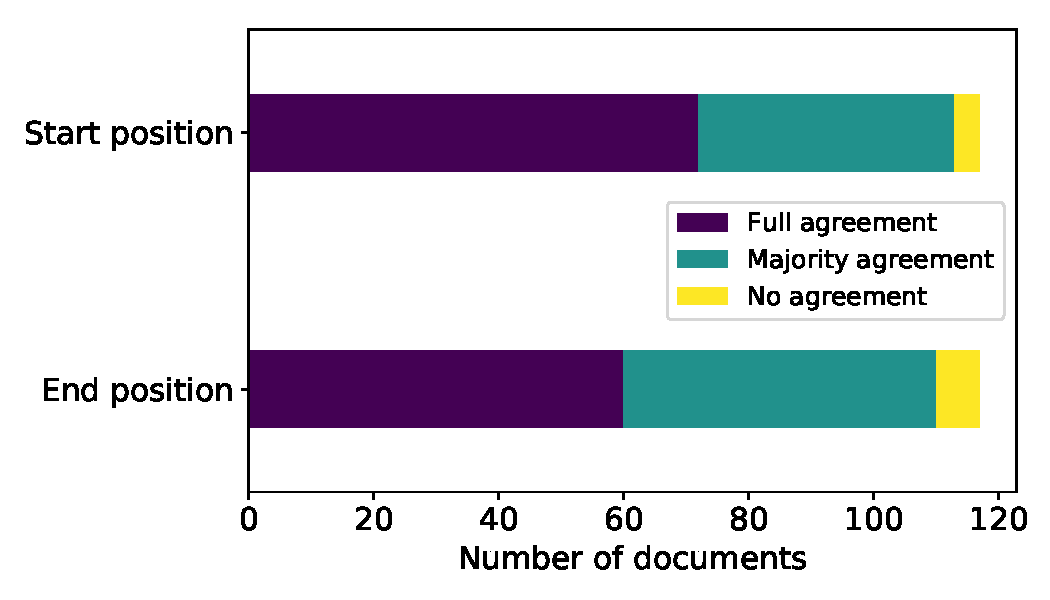
\includegraphics[width=0.5\textwidth]{annotation_agreement.pdf}
      \caption{Agreement on podcast episode introductions with annotation from three annotators. The majority of episodes have a perfect or majority agreement, and few have no agreement.}
    \label{fig:annotation_agreement}
\end{figure}

We collect the podcast transcripts using Google's speech-to-text service. The podcasts are grouped into 20 categories by topic (e.g. news, sports, comedy, etc.). To select data for annotation, we collect 3 recent episodes from the top 10 most popular podcast programs in each category, resulting in a set of 600 episodes. At the time of submission, 417 episodes have been annotated. We only keep the English podcasts and use the original transcriptions without any post-editing.

While the formats of podcasts vary, the episodes in a podcast program usually share similar topic(s) and format(s). For example, all episodes in the \emph{B\&H Photography Podcast}\footnote{\text{https://www.bhphotovideo.com/explora/podcasts}}
are about photography. All episodes in the \emph{Song Exploder}\footnote{\text{http://songexploder.net/}}
program share a similar structure: introduction, a song, and then an interview with the creator(s) of the song. Intuitively, it will be much easier for a model to perform well on given episodes if it is trained on other episodes in the same program. We therefore stratify the data, leaving 5\% of the programs out and use all episodes in these programs as ``test set of unseen programs". From the rest of programs, we further keep 10\% of their episodes as ``test set of seen programs". The rest of the dataset is used as training set. The number of episodes in the training and test sets are summarized in Table \ref{table:data_stats}.

% This allows us to control for the topics and enabling our model to learn the structural segmentation boundaries, while covering a wide variety of data to improve the extensibility of the model. 

\begin{table*}[h]
\centering
\begin{tabular}{llc}
\hline &  \textbf{Training set size} & \textbf{Test set size} \\ \hline
NeurIPS papers & 3531  & 393 \\
Podcast transcripts & 350  & 39 (seen programs)/28 (unseen programs) \\
\hline
\end{tabular}
\caption{ \label{table:data_stats} Number of documents in the training and test sets.}
\end{table*}


A group of 16 annotators were recruited to label the podcast transcripts. Each annotator listens to a podcast episode while looking at its transcript. Annotators are instructed to identify two types of introductions: the first is the \emph{program introduction}---the high-level description of a podcast program's contents, which can be similar or even identical for all episodes in a program. Second, the \emph{episode introduction}, which is a short description of a specific episode's topic, host, guest, or other important subjects discussed in it.  As the program introductions are trivial to identify, we focus on the episode introductions\footnote{Except in this paragraph, we use the word ``introductions" to indicate episode introductions in this paper.}. 

We ask the annotators to label the starting and ending words of each of these contents, or mark ``none" if they are not present. The annotators are also provided with a text box to write their comments. We do not provide a detailed guideline of what is required for an introduction, but encourage the annotators to use their own judgement in order to obtain more spontaneous reaction to the data.

The noisy and error-prone transcripts obtained from ASR data make this task challenging. When the exact beginning or ending word is mis-transcribed, an annotator may have trouble identifying them. Moreover, the time stamps of words are sometimes erroneous, making it impossible to label the exact word. Even if the transcription is perfect, two human annotators may disagree on what constitutes an introduction. Taking account of these issues, we have a number of episodes labeled by three independent annotators. At the time of submission, 117 our of the 417 total episodes have been labeled by three annotators. We define the gold standard to be majority agreement---where at least two out of three annotators have an agreement. If all three annotators agree, we consider it a perfect agreement. Because of the noise in the data, if two labels differ by less than 2 seconds, we consider them as having an agreement. 

We examine the annotator agreement on the 117 episodes with three annotations. Figure \ref{fig:annotation_agreement} shows the number of perfect and majority agreements for these episodes. For the annotations on the start of introductions, out of the 117 episodes, 72 have perfect agreement---i.e. all annotators agree on the same start position. Forty-one episodes have majority agreement, and only 4 have no agreement. If we only consider episodes with perfect or majority agreement, we obtain 113 episodes or 96.6\% of the data. Similarly, considering also the agreement on the end position, we are left with 110 episodes or 94.0\% of the data. For the podcast programs with 100\% annotator agreement, we include all episodes in these programs in the dataset even if they have not been labeled by three independent annotators.

% We also consider the accuracy of annotators by comparing each of their annotations with the gold standard. We find the average accuracy of annotators to be 91.9\%, which we use as the standard for human performance. 



\begin{figure}[ht!]
  \centering
  \vspace{-0.4cm}
    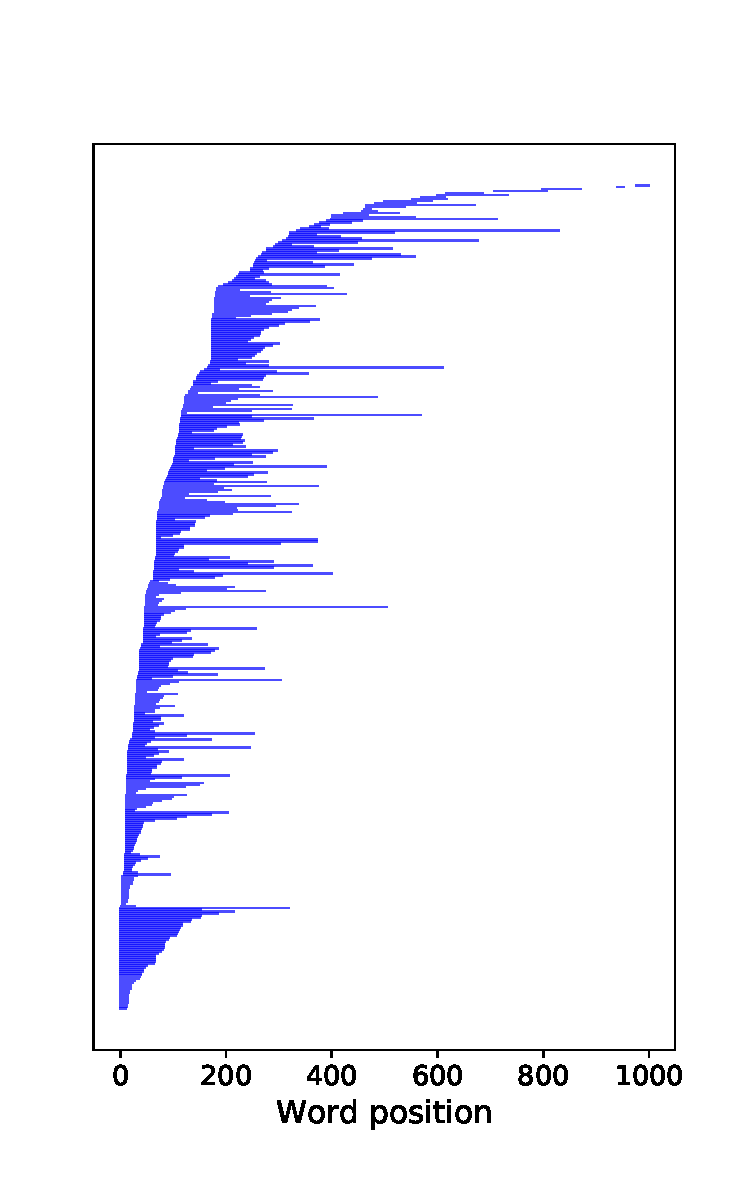
\includegraphics[width=0.5\textwidth]{start_end_position.pdf}
    \vspace{-1cm}
      \caption{Locations of episode introductions in the transcripts. Each line shows the start, end, and duration of an episode's introduction by word positions.}
    \label{fig:start_end_position}
\end{figure}


From the annotated data, we notice that the structures of podcast episodes are not consistent. For example, some episodes have program introductions before episode introductions, and vice versa. A number of episodes do not have any introductions at all. Music and advertisements may also be inserted before or after the introductions. Figure \ref{fig:start_end_position} shows the locations of episode introductions. We found these locations to vary widely, with episode introductions starting or ending as late as near 1,000 words into the transcripts.




\section{Approach} \label{sec:approach}
Our general approach to the discourse structure identification task involves two steps. First, we perform sequence labeling by training the models to make a binary classification, assigning one of two labels to each of the input tokens. In the NeurIPS task, we label each token as \texttt{Is-abstract} or \texttt{Is-body}. In the Podcast task, we label each token as \texttt{Is-intro} or \texttt{Not-intro}. We then use a boundary detector based on a maximum difference algorithm to identify the best split position(s) (see below). Each of our models has a different approach to the first part, while the algorithm for the second task is consistent across the board.

To fine-tune BERT, we first tokenize the documents using BERT's tokenizer. If a document is longer than 512 tokens, we segment it into overlapping spans because of BERT's input length limit. Following the practice in \citet{devlin2018bert}, We use a sequence length of 512 with 128 overlapping tokens between spans. The spans are re-merged after training using a maximum minimum method described in \citet{devlin2018bert}. 

\begin{figure*}
    \centering
    \begin{subfigure}[h]{0.8\textwidth}
        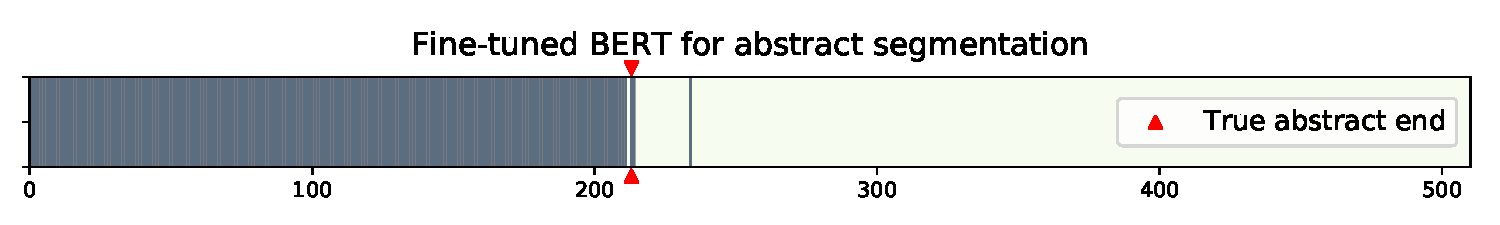
\includegraphics[width=\textwidth]{score_dist_bert_abstract.pdf}
        \vspace{-0.3in}
        \caption{}
        % \caption{Example where the fine-tuned BERT's predicted scores align well with the ground truth.}
        \label{fig:score_dist_bert_abstract}
    \end{subfigure}
    \begin{subfigure}[h]{0.8\textwidth}
        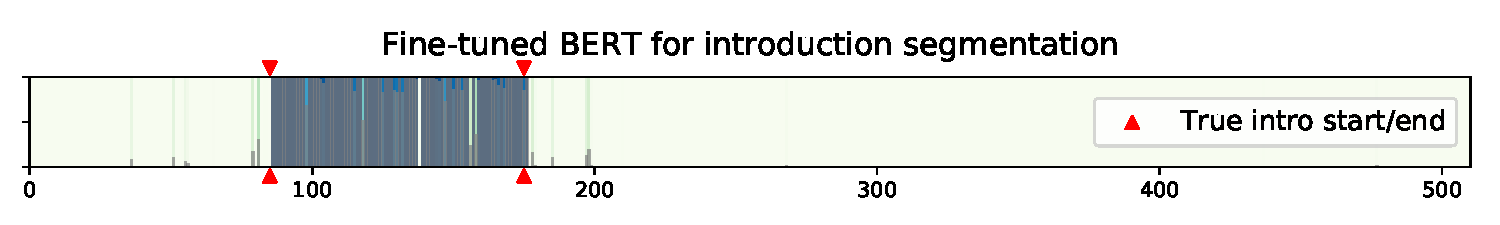
\includegraphics[width=\textwidth]{score_dist_bert_intro.pdf}
        \vspace{-0.3in}
        \caption{}
        \label{fig:score_dist_bert_intro}
    \end{subfigure}
    \begin{subfigure}[h]{0.8\textwidth}
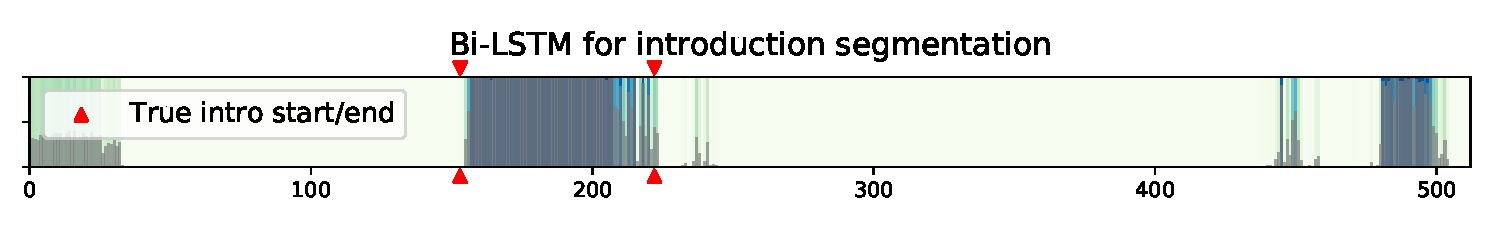
\includegraphics[width=\textwidth]{score_dist_Bi-LSTM.pdf}
        \vspace{-0.3in}
        \caption{}
        % \caption{Example where the Bi-LSTM mistakenly identifies another block of text as introduction.}
        \label{fig:score_dist_lstm}
    \end{subfigure}
    \begin{subfigure}[b]{0.8\textwidth}
        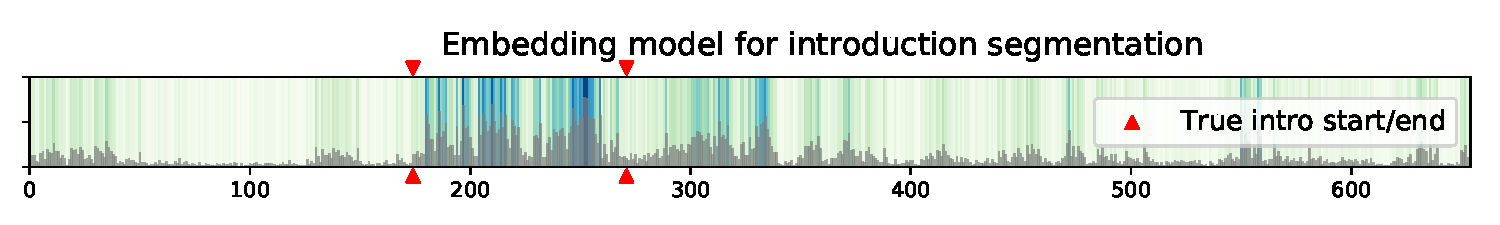
\includegraphics[width=\textwidth]{score_dist_Embedding.pdf}
        \vspace{-0.3in}
        \caption{}
        % \caption{Example where the embedding model correctly identifies the introduction, but also predicts other parts of the document as high Is-intro texts.}
        \label{fig:score_dist_embedding}
    \end{subfigure}
    \caption{Distribution of the models' prediction scores. the x-axis are the index of tokens. Each vertical line is the probability for being \texttt{Is-intro} or \texttt{Is-abstract} for a token. The darker lines indicate higher probabilities, while the gray bars show the raw probability scores. The ground truth boundaries are indicated.}\label{fig:score_dist}
\end{figure*}


We use the pre-trained BERT model \texttt{bert-base-uncased} provided in the \texttt{PyTorch Transformers} package \cite{Wolf2019HuggingFacesTS}. We train the model for 300 epochs, using the \texttt{AdamW} optimizer with an initial learning rate of $2e-5$. Linear warm-up and decay are used for learning rate adjustment. The cross entropy function is used as the loss function.

The RNN model uses a similar preprocessing and training strategy. We use a Bi-LSTM model with 64 hidden LSTM units on each direction. Inputs are first passed through a pre-trained embedding layer of GloVe vectors \cite{pennington2014glove}, and then the LSTM layer. We use the \texttt{AdamW} optimizer and learning rate $0.005$, as well as the cross entropy loss function.

For the embedding-based baseline, we extract the word embeddings using the same pretrained BERT model. The sum of the last 4 hidden layers are used to obtain word embeddings for each token in the training and test sets, following a practice in \cite{devlin2018bert}.  We then train a logistic classifier to label each token.

Our models label each token based on a predicted probability score between $0$ and $1$. As a result, the tokens predicted with high \texttt{Is-intro} or \texttt{Is-abstract} probabilities may be found throughout a document (see Figure \ref{fig:score_dist}). We therefore create a simple maximum difference algorithm to identify the best segmentation boundaries. For example, we evaluate how likely each token is the introduction's start position by looking at the tokens before and after it:

\begin{equation}
P_i = \frac{\sum_{n=1}^k{S_{i+n}}}{k} - \frac{\sum_{n=1}^k{S_{i-n}}}{k}
\end{equation}
where $P_i$ is the likelihood for a token to be the start position, $S_i$ is the \texttt{Is-intro} score assigned by our model, and $k$ is a chosen window size. For instance, if $k=20$, for each token $i$, we calculate the average \texttt{Is-intro} score for the 20 tokens before and after $i$. The token $i$ that maximizes $P_i$ is chosen as the introduction start position. We select the introduction end position and the abstract segmentation position in a similar manner.


% The architecture of our model is shown in Figure \ref{fig:model}. 
% \begin{figure*}
%   \centering
%     \includegraphics[width=\textwidth]{bert_model.png}
%       \caption{Model architecture}
%     \label{fig:model}
% \end{figure*}

\begin{figure*}
    \centering
    \begin{subfigure}[h]{0.45\textwidth}
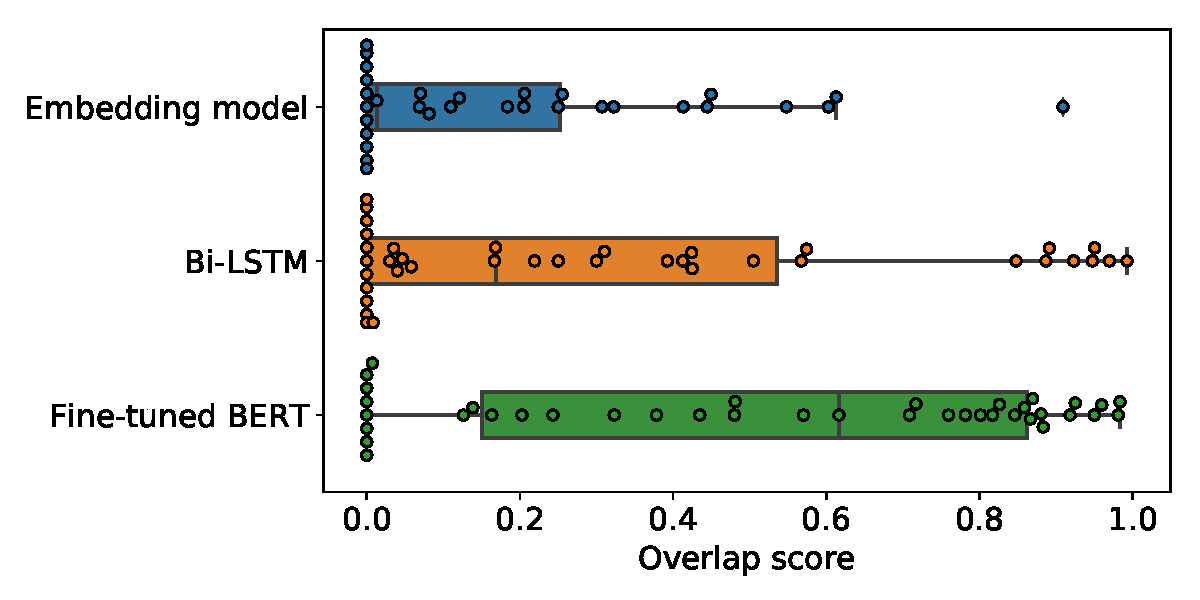
\includegraphics[width=\textwidth]{paper/figs/overlap_swarm_seen.pdf}
        \caption{Test set with seen programs.}
        \label{fig:overlap_seen}
    \end{subfigure}
    \begin{subfigure}[h]{0.45\textwidth}
        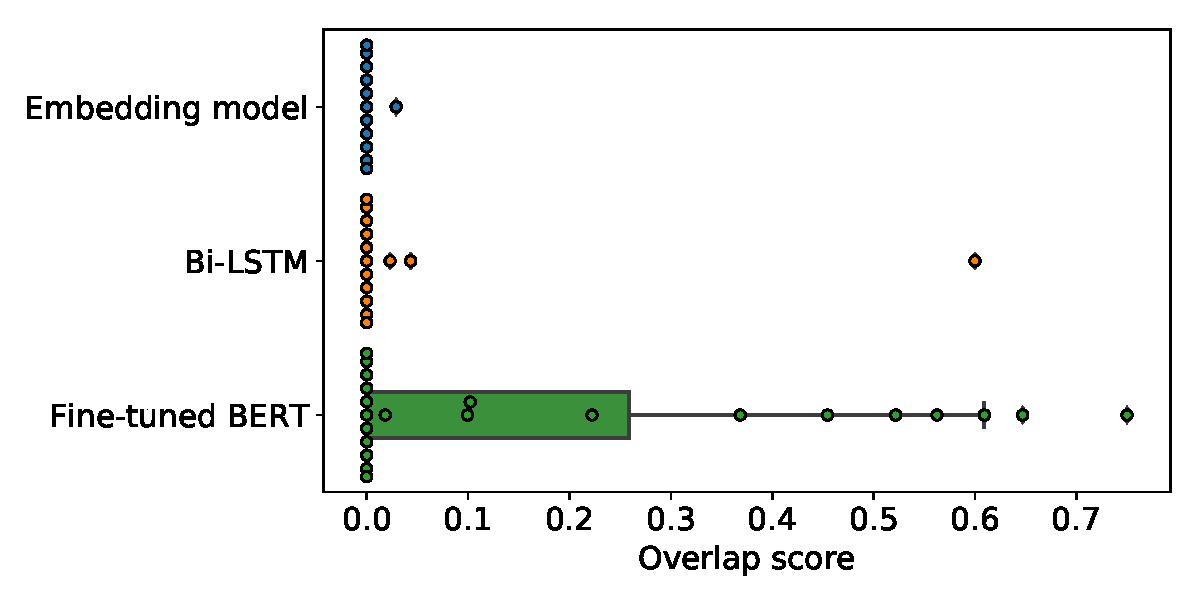
\includegraphics[width=\textwidth]{paper/figs/overlap_swarm_unseen.pdf}
        \caption{Test set with unseen programs.}
        \label{fig:overlap_unseen}
    \end{subfigure}
    \caption{Distribution of overlap scores. The x-axis shows the overlap score between 0 and 1. Each point is a document in the test sets. }\label{fig:overlap_swarm}
\end{figure*}




\section{Results}\label{sec:results}


\begin{table*}[h]
\begin{center}
\begin{tabular}{cccccc} 
\hline
\diagbox{Accuracy}{Offset} & 0 & 1 & 3 & 5 & 9\\
\hline
&&\multicolumn{2}{c}{NeurIPS task}&& \\

Fine-tuned BERT & 0.807 & 0.894 & 0.974 & 0.989 & \textbf{1.0}   \\
Bi-LSTM & \textbf{0.994} &  \textbf{0.997}  & \textbf{0.997} & \textbf{0.997} & 0.997 \\
Embedding model & 0.208 & 0.636 & 0.720  & 0.760 & 0.796   \\
\hline
&\multicolumn{3}{r}{Podcast task: seen(unseen)}&& \\
Fine-tuned BERT & \textbf{0.256(0.0)} & 0.282(0.0) & \textbf{0.410(0.179)} & \textbf{0.462(0.428)} & \textbf{0.538(0.464)} \\
Bi-LSTM & 0.0(0.0) & \textbf{0.333(0.0)} & 0.333(0.036) & 0.359(0.071) & 0.461(0.107)\\
Embedding model & 0.026(0.0) & 0.102(0.0) & 0.128(0.0) & 0.231(0.036) & 0.256(0.036) \\
\hline
\end{tabular}
\caption{Accuracy versus offset, where the offset is how many tokens there are between the predicted position and the true position. For Podcast Introductions, the results on test set of unseen programs are shown in parenthesis.}
\label{table:start_acc}
\end{center}
\end{table*}

 
We first show the alignment between the models' predictions and the ground truth. Figure \ref{fig:score_dist} shows four examples of our models' predictions. A model is performing well if its predictions align well with the ground truth. In general, all models are able to correctly label some blocks of text. In Figure \ref{fig:score_dist_bert_abstract}, the fine-tuned BERT model is able to cleanly separate the abstract and body text, despite incorrectly labeling one token in body text with high \texttt{Is-abstract} probability. In Figure \ref{fig:score_dist_bert_intro}, the model identifies the podcast introduction with a high accuracy. Similarly, in Figure \ref{fig:score_dist_lstm}, the Bi-LSTM model labels the introduction correctly, but also labels a non-relevant block of text with high \texttt{Is-intro} probability. In Figure \ref{fig:score_dist_embedding}, the embedding-based baseline appears to have more false positives, predicting more high \texttt{Is-intro} scores beyond the end of the true introduction.

With a general understanding of the models' behaviour, we formally evaluate our model's performance by two metrics inspired by the practice in \citet{rajpurkar2016squad}. First, we examine the accuracy in predicting the segmentation boundaries. We consider the accuracy in regard to given offsets, i.e. how far away the predicted boundary is from the ground truth. For the abstract segmentation task, we focus on the boundary between the abstract and body text. In the introduction segmentation task, we focus on the introduction start position, as it is often more useful to identify the start of introduction than the end. The accuracy corresponding to varied offset is shown in Table \ref{table:start_acc}. 

We found that all models perform well in the NeurIPS task. While the Bi-LSTM model achieves very high accuracy with offset $=$ 0 (i.e. exactly correct prediction), the fine-tuned BERT model has a slight advantage with a larger offset, reaching 100\% accuracy at offset $=$ 9. Both models outperform the lexical baseline by over 20\%. In the Podcast task, the fine-tuned BERT model generally outperforms the Bi-LSTM model as well as the baseline both on the test set with seen programs and that with unseen programs. At offset $=$ 0, it is able to achieve over 25\% accuracy on test set with seen programs, and over 53\% accuracy with offset $=$ 9. On the test set of unseen programs, it is the only model to achieve over 40\% accuracy with offset $=$ 9. We notice that while the Bi-LSTM model's performance is close to the BERT model on the test set with seen programs, and even overtakes BERT in one case, its accuracy is much lower on the test set with unseen programs.


 We also evaluate performance on the Podcast task with an additional metric---the overlap between the predicted introduction and true introduction on a token level. Because good predicted introductions need to not only contain the right tokens, but also be at the correct position, it is not suitable to compute the F1 score using a bag-of-tokens model. We compute the overlap score as:

\begin{equation}
S = \frac{\textrm{predicted intro} \cap \textrm{true intro} }{\textrm{predicted intro} \cup\textrm{true intro}}
\end{equation}

The overlap score distribution of our models are summarized in Figure \ref{fig:overlap_swarm}. We found that all models' results have a number of episodes with 0 overlap score, which is often caused by the models being unable to find the start or end of introduction in a document. Meanwhile, in both of the test sets, the fine-tuned BERT model has the largest number of episodes with non-zero overlap scores, and has a much higher median and $75^{th}$ percentile score than the other two models, as well as a number of episodes with near 1.0 overlap score. The Bi-LSTM model outperforms the baseline on the test set of seen programs, but its performance is not significantly different from the baseline on that of unseen programs.



\section{Analysis} \label{sec:analysis}

The fine-tuned BERT model's good performance is not surprising, but we could not directly observe how BERT learns to make such predictions. In this section, to explain BERT's performance, we look into the model's hidden layers. We first visualize the model's attention weights before and after training. The weights in each of the 12 attention heads in each of the 12 layers are plotted using the \texttt{bertviz} tool \cite{vig2019transformervis}. We notice that before fine-tuning, the attention heads have several categories of typical patterns, such as attending to the [SEP] symbols or to the next word, as described in e.g. \citet{clark2019does}. However, after fine-tuning, many of these patterns have diluted. Meanwhile, some of the attention heads appear to have learned to attend to the segmentation boundaries. For example, Figure \ref{fig:bert_attention} shows the weights in one attention head in our fine-tuned model. We notice that the model has learned a strong weight for the word ``today", which is the beginning of the introduction in this sequence.


\begin{figure}
  \centering
    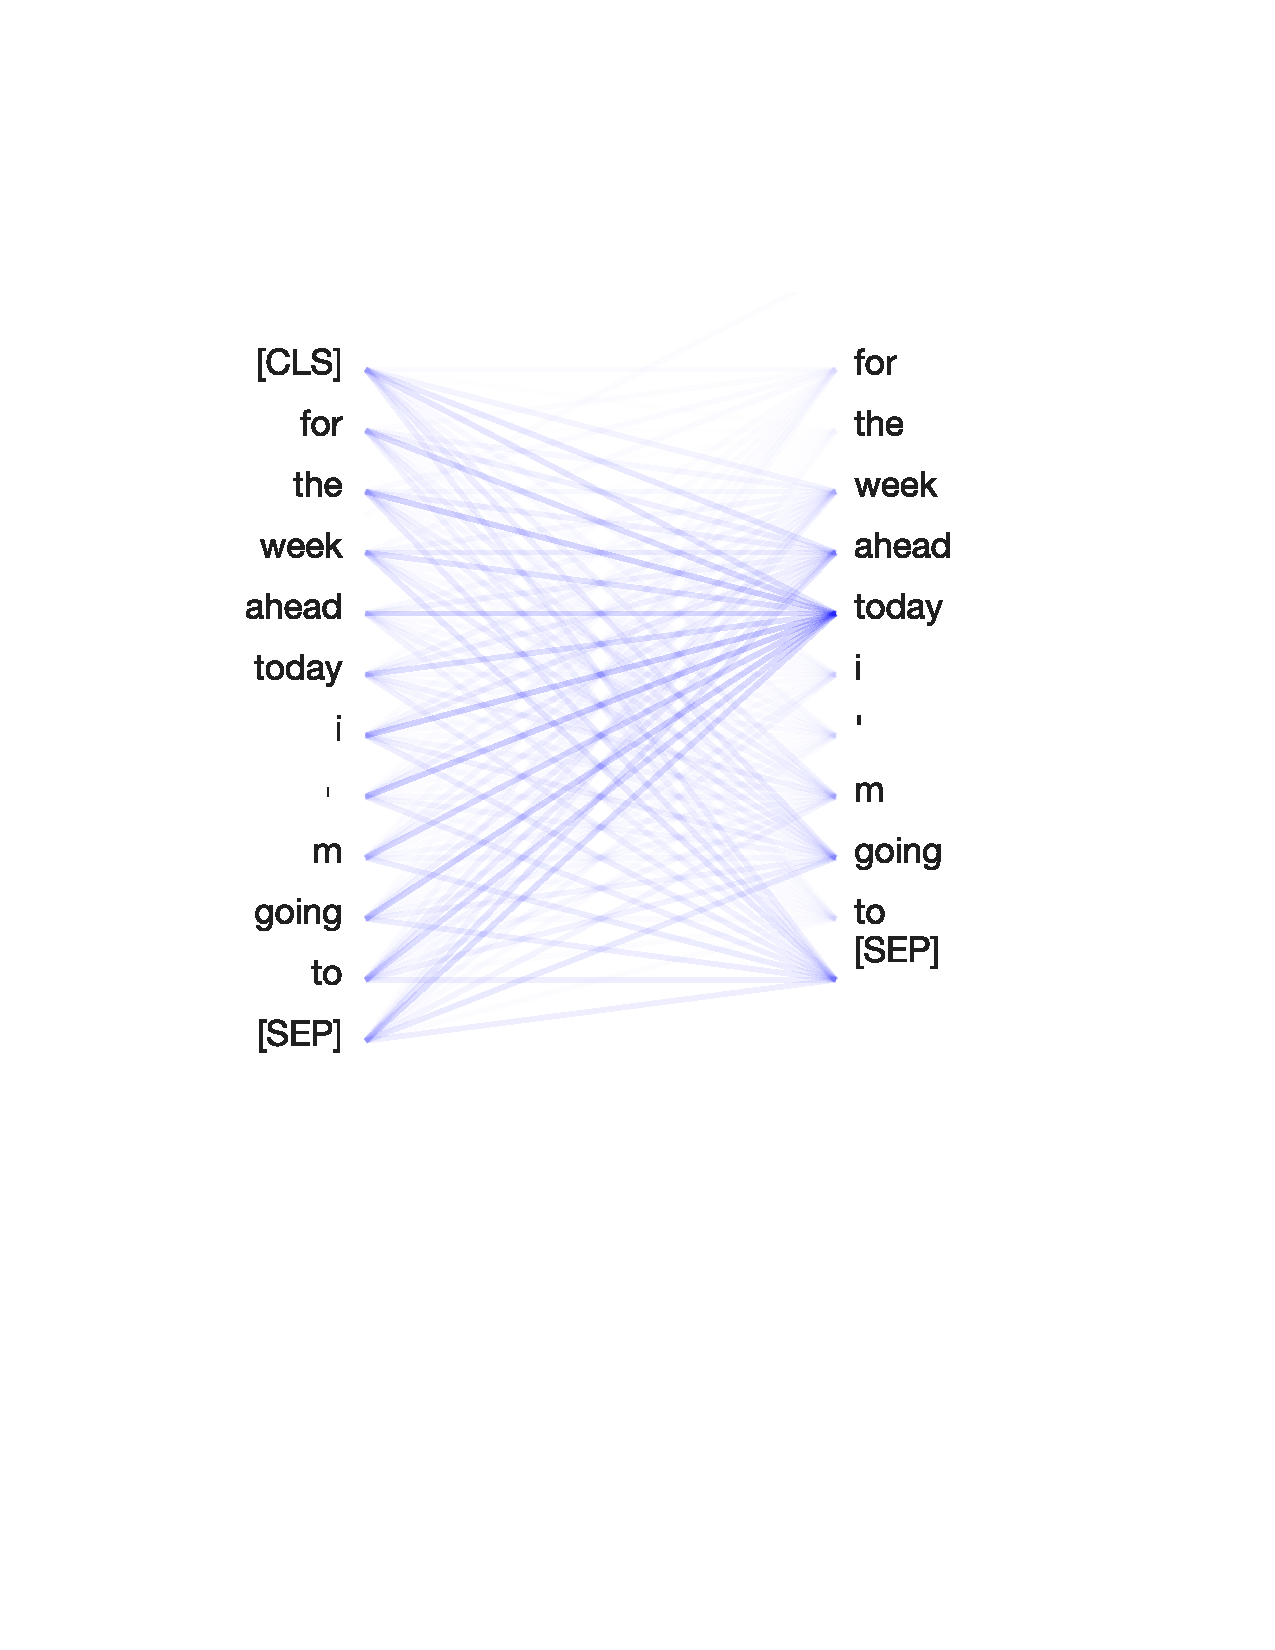
\includegraphics[width=0.48\textwidth]{paper/figs/neuron_view_bert_rm_lines.pdf}
    \vspace{-0.1in}
      \caption{Attention weights of layer 1, head 4 in the fine-tuned BERT model on a sequence extracted from a podcast transcript. Darker lines indicate stronger attention weights. The introduction starts at the word ``today".}
    \label{fig:bert_attention}
\end{figure}

To better understand the information that the model has learned, we further examine the hidden representations that the model learns for the input tokens. We extract the output of each hidden layer as learned vector representations. Inspired by the method used in \cite{van2019does}, we perform a principal component analysis (PCA) on the output vectors, which have 768 dimensions each, for dimensionality reduction. We then plot the tokens using the first two principal components. In this way, we expect to find clusters of tokens that the fine-tuned BERT model consider to be closely related. Figure \ref{fig:bert_layers} shows the token clustering from output of layer 1 and layer 12. We found that in layer 1, words with similar syntactic functions are close to each other; for example, there is a cluster of verbs on the upper left corner and one of auxiliary verbs on the right. Meanwhile, there is no separation between the \texttt{Is-intro} or \texttt{Not-intro} tokens. However, at layer 12, two distinct clusters appear, containing the \texttt{Is-intro} and \texttt{Not-intro} tokens respectively. This is consistent with the findings in \citet{van2019does} and \citet{tenney2019bert}, where the lower and higher layers in BERT are found to contain different types of information. In the lower layers, such as layer 1, the model learns and maintains syntactic representation, while the higher layers focus on task-specific information. We speculate that such learning phrases allow the BERT model the versatility to learn structural information in addition to lexical and topic information.


\begin{figure}
    \centering
    \begin{subfigure}[h]{0.5\textwidth}
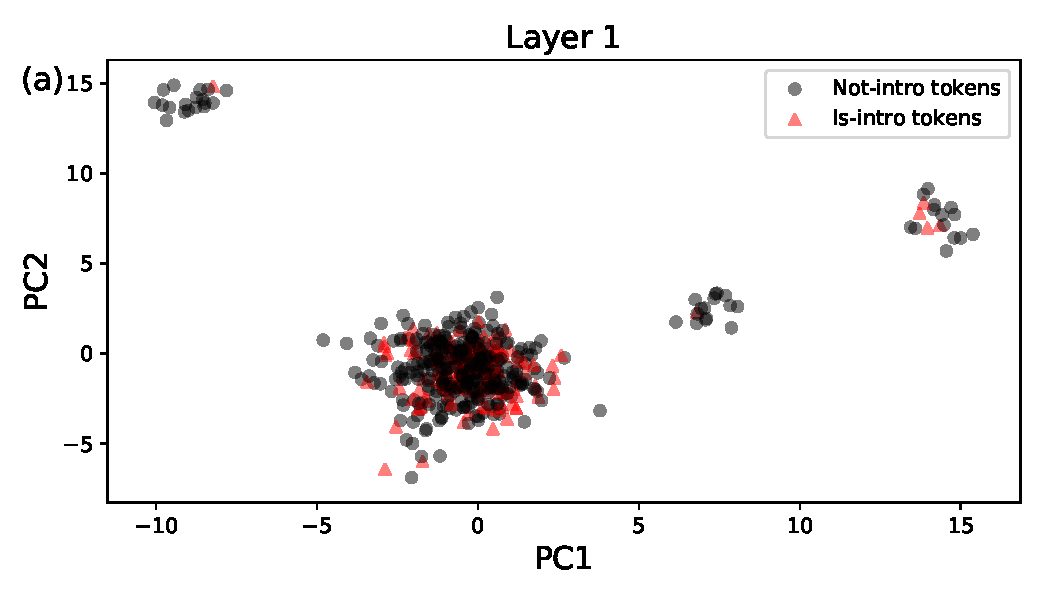
\includegraphics[width=\textwidth]{paper/figs/bert_pca_layer1_sm.pdf}
        % \caption{}
        \label{fig:bert_layer_1}
    \end{subfigure}
    \begin{subfigure}[h]{0.5\textwidth}
        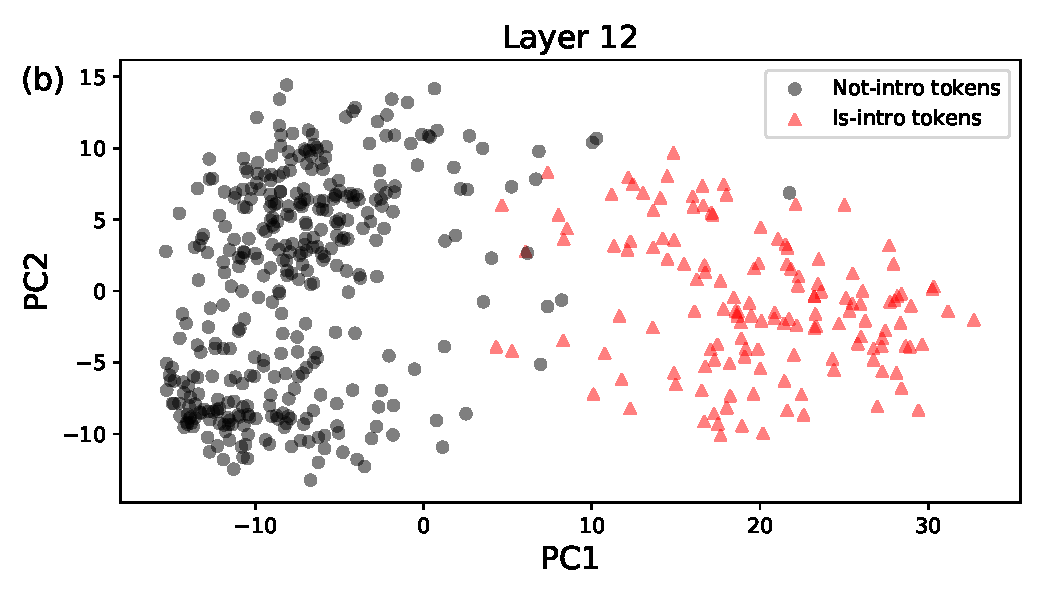
\includegraphics[width=\textwidth, ]{paper/figs/bert_pca_layer12_sm.pdf}
        % \caption{}
        \label{fig:bert_layer_12}
    \end{subfigure}
    \caption{Token clustering from BERT outputs. (a) output of layer 1. (b) output of layer 12. Red markers show the \texttt{Is-intro} tokens, and black show the \texttt{Not-intro} tokens.}
    \label{fig:bert_layers}
\end{figure}


\section{Discussion}\label{sec:discussion}

%% New (monday):

In this work, we have developed an approach to segment text data based on macro-level discourse structure using sequence models. While both of our models---Bi-LSTM and BERT---perform very well on the NeurIPS task, it is much harder to achieve high accuracy on the Podcast task. We suspect that the NeurIPS task is simpler due to the highly regular rhetorical structure of scientific paper abstracts. A good abstract mirrors the construction of a paper, as currently construed in scientific literature. The abstract will begin with an outlay of the field of study, the questions to be addressed, mentions of related work, then continues with a brief identification of methods and data, and ends with a statement of conclusions and results. 

Perhaps because the structure of this type of discourse is so fixed, the transition from the abstract to the longer introduction within the paper itself is easier to identify. In the Podcast task, the structure of the introduction segment is both less fixed by convention, and more variable across different podcast genres. Although we did find that some programs had very regular introduction structure (e.g. {\it Song Exploder}), many had a looser, more conversational style, without a standardized structure.

Transcription noise is also a factor in the podcast dataset, as is the fundamental difference between written and speech data. While the written NeurIPS texts are well-edited, the speech data is generally less organized, and also error-prone, with restarts, disfluencies, and interruptions. All of these may be reasons why a complex model like BERT is needed to capture the structures in the podcast data.

% This irregular nature of the captured data poses more challenges for future work related to spoken discourse.

On the Podcast task, while the fine-tuned BERT model and Bi-LSTM model have similar performance on the test set of seen programs, the BERT model significantly out-performs the Bi-LSTM model on the test set of unseen programs. This demonstrates BERT's ability to extend to unfamiliar data, as well as suggests the existence of some embedded linguistic and structural knowledge, which the model is able to generalize across different introduction structures. Such knowledge appears to be only identifiable to BERT, and not the simpler models. We speculate this is because BERT's multiple attention layers allow it to learn and maintain richer syntactic, semantic, and task-specific information. Although we are able to recognize some of this information captured in the model's attention architecture, we have yet to fully understand how the model is able to learn it. A future direction of our work is to provide further explanation of these models' behaviour.

%\section{Appendices}
% \label{sec:appendix}


%\section{Supplemental Material}
% \label{sec:supplemental}


\bibliographystyle{acl-natbib}
\bibliography{intro_draft.bib}

\end{document}


\begin{table}
\centering
\begin{tabular}{lrl}
\hline \textbf{Type of Text} & \textbf{Font Size} & \textbf{Style} \\ \hline
paper title & 15 pt & bold \\
author names & 12 pt & bold \\
author affiliation & 12 pt & \\
the word ``Abstract'' & 12 pt & bold \\
section titles & 12 pt & bold \\
subsection titles & 11 pt & bold \\
document text & 11 pt  &\\
captions & 10 pt & \\
abstract text & 10 pt & \\
bibliography & 10 pt & \\
footnotes & 9 pt & \\
\hline
\end{tabular}
\caption{\label{font-table} Font guide. }
\end{table}



\paragraph{\LaTeX-specific details:}
Table~\ref{citation-guide} shows the syntax supported by the style files.
We encourage you to use the natbib styles.
You can use the command {\small\verb|\citet|} (cite in text) to get ``author (year)'' citations as in \citet{Gusfield:97}.
You can use the command {\small\verb|\citep|} (cite in parentheses) to get ``(author, year)'' citations as in \citep{Gusfield:97}.
You can use the command {\small\verb|\citealp|} (alternative cite without  parentheses) to get ``author year'' citations (which is useful for  using citations within parentheses, as in \citealp{Gusfield:97}).
